% a-project.tex, v-1.0.3 marcoreis baseado no
% abntex2-modelo-trabalho-academico.tex, v-1.9.7 laurocesar
% Copyright 2012-2018 by abnTeX2 group at http://www.abntex.net.br/ 
% 
% This work consists of the files ........
% 
% -----------------------------------------------------------------------------
% Modelo para desenvolvimento de documentação de projetos acadêmicos
% (tese de doutorado, dissertação de mestrado e trabalhos de monografias em geral) 
% em conformidade com ABNT NBR 14724:2011: Informação e documentação. 
% -----------------------------------------------------------------------------
% Opções para a documentação
%
% Fancy page headings 
%\documentclass[fancyheadings, subook]{Classes/a-prj}
%\documentclass[fancyheadings, sureport]{Classes/a-prj}
%
% Fancy chapters and sections headings 
%\documentclass[fancychapter, subook]{Classes/a-prj}
%\documentclass[fancychapter, sureport]{Classes/a-prj}
%
% Fancy page , chapters and sections headings
%\documentclass[fancyheadings, fancychapter, subook]{Classes/a-prj}
\documentclass[fancyheadings, fancychapter, sureport]{Classes/a-report}
%
% -----------------------------------------------------------------------------
% Alguns comandos para a fancy page headings)
%
% Page header line width
%\footlinewidth{value}
%
% Page footer line width
%\headlinewidth{value}
%
% Page header and footer line width
%\headingslinewidth{value}
%
% Page header and footer lines without text
%\headingslinesonly
%
% The default line width is 0.3pt.
% Set the value to 0pt to remove the page header and/or footer line
%
% -------------------------------------------------------------------------------
% Formato de figuras suportado
% -------------------------------------------------------------------------------
% O formato das figuras depende da forma como o arquivo de saída é gerado.
% As figuras inseridas na pasta Figures serão automaticamente reconhecidas sem
% a necessidade de inserir a extensão do arquivo.
%
% O pdfLaTEX (PDF) suporta figuras com as extensões: pdf, jpg, png e mps.
%
% -------------------------------------------------------------------------------
% Árvore do diretório a-project.tex
%  Diretório
%       \Classes        (requerido)
%       \Figures        (requerido) --------------------------------->
%       \Figures\PDF    (optional)
%       \Figures\JPG    (optional) Figures located within these
%       \Figures\PNG    (optional) folders are searched automatically
%       \Figures\MPS    (optional)  by the a-prj class.
%       \Figures\EPS    (optional)
%       \Figures\PS     (optional) <--------------------------------
%       \Tables         (requerido)
%       \Others         (requerido)
%       \Chapters       (requerido)
%       \Appendices     (optional)
%       \References     (requerido)
%
% -------------------------------------------------------------------------------
% PDF File resumo
\ifpdf
    \hypersetup{
    	backref,
        colorlinks  = true,
        pdftitle    = Modelo de documentação,
        pdfauthor   = {Marco Reis, marco.a.reis@gmail.com},
        pdfsubject  = Mestre em Engenharia,
        pdfcreator  = Subtitulo,
        pdfproducer = PDFLatex,
        pdfkeywords = {documentação, latex, dissertação, tese}}
 \fi
%
% -------------------------------------------------------------------------------
% Relação de pacotes opcionais utilizados
\usepackage[utf8]{inputenc}
\usepackage[brazil]{babel}
\usepackage{longtable}
\usepackage{dcolumn}
\usepackage{multirow}
\usepackage{lscape}
%\usepackage{graphicx}
\usepackage{rotating}
%\usepackage{float,subfigure}
%\usepackage{graphicx, subfigure}
\usepackage{cite}
\usepackage[left=3cm,top=3cm,right=2cm,bottom=2cm]{geometry}
\usepackage[alf]{abntex2cite}
\usepackage{ifpdf}
\usepackage{shadow}
\usepackage{wrapfig}
\usepackage[normalem]{ulem}
\usepackage{makeidx}
\usepackage{yfonts}
\usepackage{algorithm}
\usepackage{algorithmic}
\usepackage{lmodern}
\usepackage[T1]{fontenc}
\usepackage{indentfirst}
\usepackage{color}
\usepackage{microtype}
\usepackage{lipsum}
\usepackage{caption}
\usepackage{subcaption}
%
\makeindex 
\setlength{\LTcapwidth}{\textwidth}
%
\newtheorem{theorem}{Teorema}
\newtheorem{definition}[theorem]{Definição}
%
% -------------------------------------------------------------------------------
% Configurações do pacote backref
\renewcommand{\backrefpagesname}{Citado na(s) página(s):~}
% Texto padrão antes do número das páginas
\renewcommand{\backref}{}
% Define os textos da citação
\renewcommand*{\backrefalt}[4]{
	\ifcase #1 %
		Nenhuma citação no texto.%
	\or
		Citado na página #2.%
	\else
		Citado #1 vezes nas páginas #2.%
	\fi
}
% 
% -------------------------------------------------------------------------------
% Início do documento raiz
\begin{document}
% Definição do título da página
    \university{Centro Universitário SENAI CIMATEC}
	%\faculty{Programa de...}
	%\school{Escola de...}
% 
    %\course{Engenharia Elétrica}
    \typework{Relatório Final}
% 
	%\course{Mestrado em Modelagem Computacional e Tecnologia Industrial}
	%\typework{Disserta\c{c}\~ao de mestrado}
	%\typework{Exame de Qualificação de Mestrado}
% 
	%\course{Engenharia Elétrica}
	%\typework{Tese de doutorado}
	%\typework{Exame de Qualificação de doutorado}
%
% -------------------------------------------------------------------------------
% Informações gerais
    \thesistitle{Desafios para o laboratorio robotica e sistemas autonomos}
    \hidevolume
    \thesisvolume{Volume 1 of 1}
    \thesisauthor{Tiago Barretto Sant'Anna}
    %\thesisauthorr{Rick Deckard}
    \thesisadvisor{Prof. Marco Reis, M.Eng.}
    %\hidecoadvisor
    %\thesiscoadvisor{Marco Reis}
    \thesismonthyear{Dezembro de 2021}
% 
    \maketitlepage
%
%//uhu seja persistente e não deixe de se apaixonar pela robótica. Vc vai longe.
% ----------------------------------------------------------------------------
% Inserir Folha de rosto, Nota de estilo, folha de assinaturas, dedicatoria
    \begin{folharosto}

\begin{center}
\theauthor \\
%\theauthorr \\
%\theauthorrr \\
%\theauthorrrr \\
%\theauthorrrrr \\
\end{center}
\ \\
\ \\
\ \\
\ \\
\ \\
\begin{spacing}{2}
   \begin{center}
   {\LARGE {\bf \thetitle}}
   \end{center}
\end{spacing}
\ \\
\ \\
\ \\
\vspace*{85mm}
% \begin{flushright}

%    \begin{list}{}{
%       \setlength{\leftmargin}{7.5cm}
%       \setlength{\rightmargin}{0cm}
%       \setlength{\labelwidth}{0pt}
%       \setlength{\labelsep}{\leftmargin}}

%       \item \thetypework apresentada ao \thefaculty, Curso de \thecourse
%       do \theuniversity, como requisito parcial para a obten\c{c}\~ao do
%       t\'itulo de {\bf \thedegreetitle}.

%       \begin{list}{}{
%       \setlength{\leftmargin}{0cm}
%       \setlength{\rightmargin}{0cm}
%       \setlength{\labelwidth}{0pt}
%       \setlength{\labelsep}{\leftmargin}}

%       \item \'Area de conhecimento: Interdisciplinar

%       \item Orientador: \theadvisor
%       \newline \hspace*{2.1cm}  %{\it \theuniversity}

%       \end{list}
%    \end{list}

% \end{flushright}
\ \\
\ \\
\ \\
\ \\
%\begin{spacing}{1.5}
   \begin{center}
   Salvador \par
   \theuniversity \par
   2020
   \end{center}
%\end{spacing}

\end{folharosto}

    %\include{Others/NotaEstilo}
    %\include{Others/FolhaAssinaturas}
    %\include{Others/dedicatoria}
    %\include{Others/agradecimentos}
%
% ----------------------------------------------------------------------------
% Resumo/abstract, sumário e siglas
    \begin{romanpagenumbers}
        \begin{thesisresumo}

    O trabalho consiste na explanação das percepções acerca dos desafios passados. Assim conta como foi desenvolvido e as táticas utilizadas para a conclusão dessa atividade. Tem como objetivo a absorção de  conhecimentos com o intuito de realizar projetos de robótica. Para isso foram realizados estudos de uma gama de conhecimentos para poder realizar as atividades, sendo entre eles programação, simulação e \textit{ROS}.

%Escreva aqui o resumo da disserta\c{c}\~ao, incluindo os contextos geral e espec\'ifico, dentro dos quais a pesquisa foi realizada, o objetivo da pesquisa, assun\c{c}\~ao filos\'ofica, os m\'etodos de pesquisa usados e as poss\'iveis contribui\c{c}\~oes que o que \'e proposto pode trazer \`a sociedade.

\ \\

% use de três a cinco palavras-chave

\textbf{Palavras-chave}: robótica, estudo, programação, simulação.

\end{thesisresumo}

        \begin{thesisabastract}
    The work consists of explaining perceptions about past challenges. So it tells how it was developed and the tactics used to complete this activity. It aims to absorb knowledge in order to carry out robotics projects. For this, studies were carried out on a range of knowledge to be able to carry out the activities, including programming, simulation and \textit{ROS}

%Escreva aqui, em ingl\^es, o resumo da disserta\c{c}\~ao, incluindo os contextos geral e espec\'ifico, dentro dos quais a pesquisa foi realizada, o objetivo da pesquisa, assun\c{c}\~ao filos\'ofica, os m\'etodos de pesquisa usados e as poss\'iveis contribui\c{c}\~oes que o que \'e proposto pode trazer \`a sociedade. 

\ \\

% use de tr�s a cinco palavras-chave

\textbf{Keywords}: robotics, study, programming, simulation.

\end{thesisabastract}

        % Make list of contents, tables and figures
        \thesiscontents
        %\pdfbookmark[1]{Lista de Tabelas}{lot} \listoftables
        %//wow se não tem tabelas vc pode colocar a linha acima em comentário
        \newpage
        %Include other required section
        %\include{Others/abbreviation}
        %\include{Others/simbolos}
        %Switch the page numbering back to the default format
    \end{romanpagenumbers}
%
% ---------------------------------------------------------------------------
% Include thesis chapters
    \parskip=\baselineskip
    \chapter{Introdução}
\label{chap:intro}

Este artigo consiste na exposição dos desafios realizados para o 
Laboratório de Robótica e Sistemas Autônomos. Assim, esses desafios foram realizados ao longo de dois meses. Esses desafios tem como principal função realizar a capacitação para pode atuar dentro do laboratório


%--------- NEW SECTION ----------------------
\section{Objetivos}
\label{sec:obj}
Os objetivos são realizar desafios de robótica, programação 
e simulação com a função de adquirir conhecimentos para poder atuar dentro do laboratório.
\label{sec:obj}

\subsection{Objetivos Específicos}
\label{ssec:objesp}
Os objetivos específicos deste projeto são:
\begin{itemize}utilizá-lo
      \item Aprender ROS e como utiliza-lo;
      \item Desenvolver habilidades de programação em Python e C++;
      \item Obter conhecimento de simulação e programação de robôs usando o Webots;
      \item Criar um package no ROS para controlar o turtlesim;
      \item Obter conhecimentos a cerca de navegação usando o Husky
  \end{itemize}

%\subsubsection*{Objetivos específicos principais}
%\label{sssec:obj-principais}


%--------- NEW SECTION ----------------------
\section{Justificativa}
\label{sec:justi}

Esse trabalho tem como função de capacitar o estudante acerca das 
ferramentas necessarias para trabalhar com robótica, sendo aprendendo 
a utilizar o framework ROS com a versão noetic, ou habilitando seu
conhecimento em programação.


%--------- NEW SECTION ----------------------
\section{Organização do documento}
\label{section:organizacao}

Este documento apresenta $5$ capítulos e está estruturado da seguinte forma:

\begin{itemize}

  \item \textbf{Capítulo \ref{chap:intro} - Introdução}: Contextualiza o âmbito, no qual a pesquisa proposta está inserida. Apresenta, portanto, a definição do problema, objetivos e justificativas da pesquisa e como este \thetypeworkthree está estruturado;
  \item \textbf{Capítulo \ref{chap:fundteor} - Fundamentação Teórica}: Explicita toda a base teorica com o qual o trabalho foi produzido, tratando das bases para a sua construção;
  \item \textbf{Capítulo \ref{chap:metod} - Materiais e Métodos}: Evidencia por qual processo foi executado o objetivo desse artigo até a obtenção dos resultados;
  \item \textbf{Capítulo \ref{chap:result} - Resultados}: Mostra o que foi obtido com a realização desse trabalho;
  \item \textbf{Capítulo \ref{chap:conc} - Conclusão}: Apresenta as conclusóes, contribuições e algumas sugestões de atividades de pesquisa a serem desenvolvidas no futuro.

\end{itemize}

    \chapter{Conceito do projeto}
\label{chap:fundteor}

Para a realização de cada desafio foi necessario se basear em uma serie de trabalhos




\section{Desafio Workbooks Python}

O desafio de Workbooks utilizando a linguagem python foi composto de 16 desafios de programação utilizando a linguagem python. Partindo dessa contexto, tudo se iniciou com o estudo de bibliotecas e python, para poder ralizar as tarefas da forma mais eficiente possivel.

\section{Desafio C++}
O desafio de C++ foi composto de três desafios de programação que utiliza a linguagem de programação C++. Portanto para a primeira tarefa foi feito um estudo matematico para a enteder como funciona o triangulo de pascal. Em seguida para a segunda tarefa foi feito um estudo combinatorio sobre permutações e depois um estudo sobre bibliotecas  com a função de realizar essas combinações de palavras de forma mais eficaz. Por fim, para a terceira foi feito um estudo acerca de bibliotecas que trabalhassem com arquivos para assim ler o codigo que estava escrito

\section{Turtlesim setpoint position}
Consiste em utilizar o software Turtlesim para através do ROS escolher 
uma posição e fazê-lo se deslocar até ela. A movimentação programada na 
Turtlesim se baseia em uma teoria principal, que é o
Dead reckoning. Dessa forma, o Dead reckoning consistem em calcular a 
distancia que falta do robô para determinando objetivo e incorporar esses
valores a sua posição e velocidade, como pode ser exemplificado na figura \ref{fig:Dead reckoning}. No caso da Turtlesim foi calculado
sua distancia usando o teormea de pitagoras e o angulo pelo qua a tartaruga
precisou virar pela trigonometria.

%imagem  https://en.wikipedia.org/wiki/Dead_reckoning

\begin{figure}[h!]
    \centering
    \caption{Dead reckoning}
    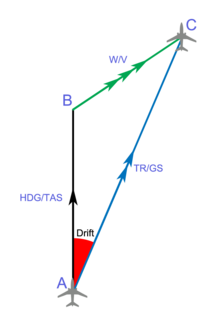
\includegraphics[width=0.8\textwidth]{Figures/dead_reck.png}
    \caption*{Fonte: WIkipedia}
    \label{fig:Dead reckoning}
\end{figure}

Na navegação do Turtlesim, o teorema de pitagoras é utilizado para calcular
a distancia entre a mesma e o objetivo definido durante cada instante. Para 
isso foi utilizado a seguinte formula 
$d = \sqrt{(x\textsubscript{f} - x\textsubscript{i})^2 + (y\textsubscript{f} - y\textsubscript{i})^2}$
. Nos quais x\textsubscript{f} e y\textsubscript{f} são as distancias finais
e x\textsubscript{i} e y\textsubscript{i} são as distancias da tartaruga 
em determinado instante.

Assim, para calcular quanto que o Turtlesim precisa girar faz o uso da 
trigonometria, para calcular o angulo do qual a Turtlesim esta deslocada 
em relação ao objetivo. Com isso, se faz o uso da formula de arctg na qual 
$\theta = \frac{y\textsubscript{f} - y\textsubscript{i}}{x\textsubscript{f} - x\textsubscript{i}} $
. Por fim, pegamos esse angulo e subtraimos do angulo atual da Turtlesim
para descobrir o quanto a tartaruga precisa rotacionar.

Para definir a velocidade da tartaruga multiplicamos a distancia por uma constante e
para descobrir o quanto ela precisa rotacionar multiplicamos a 
angulação por outra constante. Assim esses dados são publicados no topic
cmd\_vel para alterar a velocidade da turtle até que ela chegue no objetivo
especificado.

\section{Desafio Webots}

O Webots é uma plataforma opensource usada para simular robôs. 
Desse modo, o desafio consiste em utilizar essa plataforma para 
simular um robo chamado piooner3x, corringindo o codigo ja existente
e alterando ele para caso ele encontre uma luminaria pare de se locomover.

A partir disso foram realizados os tutorias dessa plataforma para 
ter conhecimento de como a utiliza-la e como simular os robos. 
Em seguida foi colocado um sensor de luz no piooner3x para que 
o mesmo tenha uma forma de detectar a luminosidade do ambiente
e seu codigo foi alterado para que se a leitura do sensor 
ultrapasse determinado valor ele pare


\section{Desafio Husky}
Husky é um veiculo UGV no qual atraves do ROS pode ser 
simulado em conjunto com o gazebosim e o rviz, sendo ambos
simualdores no qual o primeiro é voltado para o ambiente 
ao redor do husky e o segundo é como esse ugv percebe o mundo.
O desafio consiste em utilizar os simuladores para testar
diferentes formas de navegação com o husky.

O primeiro desafio é simular o husky com o package move base. 
Consiste em dar uma localização no mundo e ele ira tentar atingir 
esse objetivo. Caso o ugv identifique algum obstaculo ele ira desviar,
ou caso fique preso ira entrar em um processo chamado conservative reset
se parar de ficar preso voltara a navegação, caso não entrara em 
clearing rotation, se mesmo assim continuar preso iniciara um agressive reset
e continuando preso vai por fim fazer uma clearing rotation e se mesmo 
assim continuar preso vai abortar a ação. Como mostra na imagem

%imagem https://wiki.ros.org/move_base

O segundo desafio é o amcl demo, o qual é a junção do move base com o
amcl. Assim o amcl é um sistema probabilistico de localização do robô
o qual atraves de sensores de laser fazem o tracking da posisção do 
robo dentro de um mapa.

%imagem do simulador 

Gmapping demo é o terceiro desafio, ele é a junção do move base com o
gmapping. Esse package prove um SLAM (Simultaneos localization and mapping), 
baseado em sensores a laser. Com o gmapping é criado um mapa 2D do ambiente.
Como pode ser mostrado na imagem abaixo.

%imagem do mapa

Por ultimo foi realizado o frontier exploration demo, é composto 
pelo move base, gmapping, e o frontier exploration. Dessa forma,
o frontier em conjunto com esses packages para realizar a 
exploração de ambientes

%----------------------------------------------------------

%--------- NEW SECTION ----------------------


%---------------picture------------------------------------
% \begin{figure}
%     \centering
%     \subfigure[Figure A]{\label{fig:a}\includegraphics[width=60mm]{./lq}}
%     \subfigure[Figure B]{\label{fig:b}\includegraphics[width=60mm]{./lq}}
%     \subfigure[Figure C]{\label{fig:c}\includegraphics[width=\textwidth]{./lq}}
%     \caption{Three simple graphs}
%     \label{fig:three graphs}
% \end{figure}
%----------------------------------------------------------

% \begin{figure}
%     \centering
%     \begin{subfigure}[b]{0.3\textwidth}
%         \centering
%         \includegraphics[width=\textwidth]{./lq}
%         \caption{$y=x$}
%         \label{fig:y equals x}
%     \end{subfigure}
%     \hfill
%     \begin{subfigure}[b]{0.3\textwidth}
%         \centering
%         \includegraphics[width=\textwidth]{./lq}
%         \caption{$y=3sinx$}
%         \label{fig:three sin x}
%     \end{subfigure}
%     \hfill
%     \begin{subfigure}[b]{0.3\textwidth}
%         \centering
%         \includegraphics[width=\textwidth]{./lq}
%         \caption{$y=5/x$}
%         \label{fig:five over x}
%     \end{subfigure}
%        \caption{Three simple graphs}
%        \label{fig:three graphs}
% \end{figure}


% %--------- NEW SECTION ----------------------
% \section{Assunto 2}
% \label{sec:ass2}
% flkjasdlkfjasdlkfjs

% \begin{table}[h]
%     \begin{subtable}[h]{0.45\textwidth}
%         \centering
%         \begin{tabular}{l | l | l}
%         Day & Max Temp & Min Temp \\
%         \hline \hline
%         Mon & 20 & 13\\
%         Tue & 22 & 14\\
%         Wed & 23 & 12\\
%         Thurs & 25 & 13\\
%         Fri & 18 & 7\\
%         Sat & 15 & 13\\
%         Sun & 20 & 13
%        \end{tabular}
%        \caption{First Week}
%        \label{tab:week1}
%     \end{subtable}
%     \hfill
%     \begin{subtable}[h]{0.45\textwidth}
%         \centering
%         \begin{tabular}{l | l | l}
%         Day & Max Temp & Min Temp \\
%         \hline \hline
%         Mon & 17 & 11\\
%         Tue & 16 & 10\\
%         Wed & 14 & 8\\
%         Thurs & 12 & 5\\
%         Fri & 15 & 7\\
%         Sat & 16 & 12\\
%         Sun & 15 & 9
%         \end{tabular}
%         \caption{Second Week}
%         \label{tab:week2}
%      \end{subtable}
%      \caption{Max and min temps recorded in the first two weeks of July}
%      \label{tab:temps}
% \end{table}
    \chapter{Desenvolvimento do projeto}
\label{chap:metod}

Durante esta seção sera descrito o processo de construção dos desafios, incluindo os estudos necessarios para cada um, o processo de criação e especificidades. Será apresentado estas características para cada um desafio.

\section{Desafio Workbooks Python}

Para realização deste desafio foi realizado a pesquisa sobre bibliotecas em python para cada tarefa propria e em seguida criação de scripts e testes. Para dessa forma comcluir o desafio.

\section{Desafio C++}

Tem como inicio o estudo da linguagem C++ através da Code Academy com o seu curso. Depois, para cada tarefa foi realizado uma pesquisa propria, sendo sobre matematica teoria ou bibliotecas dessa linguagem. Assim, foi realizado o desafio.

\section{Turtlesim setpoint position}

O desafio se iniciou com um estudo sobre o ROS, mais especificamente sobre publisher e subscriber. Após isso, foi feito uma pesquisa acerca das tecnicas de navegação chegando no dead reckoninig. Em seguida, iniciou-se a fase de estudo da programação e testes do package ate chegar no produto final.

\section{Desafio Webots}

Em primeira etapa foram realizados os tutoriais do Webots, logo em diante foi feito um estudo da programação nesta plataforma. Depois disso foram realizados seguidos testes e alterações ate que o robo conseguisse se locomover corretamente para apos isso implementar o sensor de luz.

\section{Desafio Husky}

O desafio foi realizado com o uso do ROS Noetic. Para ser realizado foi feito \textit{git clone} de um repositorio no github do Husky em um workspace. Com isso, foi realizados os desafios porem alguns erros surgiram, mas foram solucionados atraves de pesquisa e ajuda de colegas.


% %--------- NEW SECTION ----------------------
% \section{Interface do Usuário}
% \label{sec:ui}
% \lipsum[1]

% %--------- NEW SECTION ----------------------
% \section{Simulação do sistema}
% \label{sec:sim}
% \lipsum[2-4]


    \chapter{Resultados}
\label{chap:result}
Depois de finalizados os desafios foram coletados os seus resultados e disponibilizados no github.

\section{Desafio Workbooks Python}

Com a conclusão do desafio, os codigos foram testados e tiveram sucesso no seu funcionamento. Assim, 

\section{Desafio C++}

Os códigos foram compilados e executados obtendo sucesso no seu funcionamento. O primeiro

\section{Turtlesim setpoint position}

Depois de finalizado o package tinha seu funcionamento como exigia o regulamento. Portanto as coordenadas eram digitadas e a tartaruga realizava um deslocamento ate alcançar uma distância de pelo menos 0.1 do objetivo e assim encerrava seu programa.

\section{Desafio Webots}

Após o explicitado na metodologia o robô piooner3x conseguiu seguir o percurso sem grandes problemas. Desse modo e parar quando encontrava uma fonte luminosa, sendo no caso uma luminária em um canto do mapa dentro de XX segundos

\section{Desafio Husky}

As diferentes navegações foram corretamente executadas e colocadas em prática dentro dos simuladores gazebosim e rviz. Com isso foi capaz perceber como as diferentes técnicas de navegação aplicadas e combinadas afetam o deslocamento do ugv




    \chapter{Conclusão}
\label{chap:conc}

Durante todos os desafios foram exigidos o aprendizado e dominio de novas ferramentas. Os desafios foram compostos de uma serie de desafios envolvendo programação, simulação, navegação e dominio do \textit{ROS}. 

%Chegou a hora de apresentar o apanhado geral sobre o trabalho de pesquisa feito, no qual s\~ao sintetizadas uma s\'erie de reflex\~oes sobre a metodologia usada, sobre os achados e resultados obtidos, sobre a confirma\c{c}\~ao ou recha\c{c}o da hip\'otese estabelecida e sobre outros aspectos da pesquisa que s\~ao importantes para validar o trabalho. Recomenda-se n\~ao citar outros autores, pois a conclus\~ao \'e do pesquisador. Por\'em, caso necess\'ario, conv\'em cit\'a-lo(s) nesta parte e n\~ao na se\c{c}\~ao seguinte chamada \textbf{Conclus\~oes}.


\section{Considerações finais}
\label{sec:consid}

O trabalho fomentou um aprendizado especifico de maneira pratica e objetiva, voltado para a criação de habilidades, o desenvolvimento do pensamento logico para resolução de problemas e absorção das ferramentas utilizadas 

Sendo assim, essas ferramentas são de grande importância para o trabalho e desenvolvimento em robótica

%Brevemente comentada no texto acima, nesta se\c{c}\~ao o pesquisador (i.e. autor principal do trabalho cient\'ifico) deve apresentar sua opini\~ao com respeito \`a pesquisa e suas implica\c{c}\~oes. Descrever os impactos (i.e. tecnol\'ogicos,sociais, econ\^omicos, culturais, ambientais, políticos, etc.) que a pesquisa causa. N\~ao se recomenda citar outros autores.


    % include more chapters ...
%
% ----------------------------------------------------------------------------
% Include thesis appendices
    \begin{thesisappendices}
        % \include{Appendices/diagmec}
        % \include{Appendices/diagele}
        %\include{Appendices/logbook}
    \end{thesisappendices}
%
%//wow vc não tem apêndices então basta comentar
% ----------------------------------------------------------------------------
% Configurar as referencias bibliograficas
	\renewcommand\bibname{Referências}
    \addcontentsline{toc}{chapter}{Referências}
    \bibliography{References/referencias}
%
% ----------------------------------------------------------------------------
% Finishing him
    \include{Others/ultimafolha}
\end{document}
%
% -------------------------------------------------------------------------------
% Aqui termina a formatação para o documento.
% In God We Trust. All Other Bring Data. 
%
% -------------------------------------------------------------------------------